\documentclass[border=4pt]{standalone}
\usepackage{mathptmx}
\usepackage{amsmath}
\usepackage{tikz}
\usetikzlibrary{positioning,arrows.meta,fit,backgrounds}
\begin{document}
\begin{minipage}{3.5in}
\resizebox{\linewidth}{!}{%
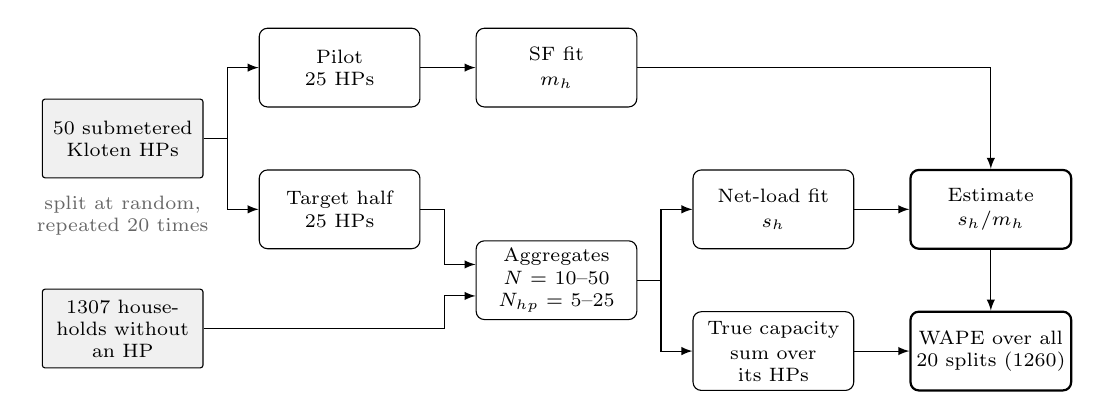
\begin{tikzpicture}[font=\scriptsize, >=latex,
  io/.style={draw, fill=black!6, rounded corners=1pt, align=center, text width=19mm, minimum height=10mm, inner sep=2pt},
  proc/.style={draw, rounded corners=3pt, align=center, text width=19mm, minimum height=10mm, inner sep=2pt},
  res/.style={draw, thick, rounded corners=3pt, align=center, text width=19mm, minimum height=10mm, inner sep=2pt},
  lab/.style={font=\scriptsize, text=black!60, align=center},
  node distance=5mm and 7mm]
% inputs
\node[io] (hps) {50 submetered Kloten HPs};
\node[io, below=14mm of hps] (free) {1307 households without an HP};
% split
\node[proc, right=of hps, yshift=9mm] (pilot) {Pilot\\25 HPs};
\node[proc, right=of hps, yshift=-9mm] (half) {Target half\\25 HPs};
\draw[->] (hps.east) -- ++(3mm,0) |- (pilot.west);
\draw[->] (hps.east) -- ++(3mm,0) |- (half.west);
\node[lab, below=1mm of hps] {split at random,\\repeated 20 times};
% pilot branch
\node[proc, right=of pilot] (sffit) {SF fit\\[1pt]$m_h$};
\draw[->] (pilot) -- (sffit);
% target branch
\node[proc, right=of half, yshift=-9mm] (agg) {Aggregates\\$N$ = 10--50\\$N_{hp}$ = 5--25};
\draw[->] (half.east) -- ++(3mm,0) |- ([yshift=2mm]agg.west);
\draw[->] (free.east) -| ([xshift=-4mm,yshift=-2mm]agg.west) -- ([yshift=-2mm]agg.west);
\node[proc, right=of agg, yshift=9mm] (netfit) {Net-load fit\\[1pt]$s_h$};
\node[proc, right=of agg, yshift=-9mm] (truth) {True capacity\\[1pt]sum over its HPs};
\draw[->] (agg.east) -- ++(3mm,0) |- (netfit.west);
\draw[->] (agg.east) -- ++(3mm,0) |- (truth.west);
% estimate and score
\node[res, right=of netfit] (est) {Estimate\\[1pt]$s_h / m_h$};
\draw[->] (netfit) -- (est);
\draw[->] (sffit.east) -| (est.north);
\node[res, right=of truth] (score) {WAPE over all\\20 splits (1260)};
\draw[->] (est) -- (score);
\draw[->] (truth) -- (score);
\end{tikzpicture}%
}
\par\smallskip
{\footnotesize Fig.~X.\ One split of the Kloten experiment. The pilot half gives $m_h$; aggregates drawn from the other half and the households without an HP give $s_h$ and their true capacity. No HP serves both the pilot and a target.}
\end{minipage}
\end{document}
